\documentclass[class=report,crop=false]{standalone}
\usepackage[screen]{../exo7book}

% Commande ponctuelle
\newcommand{\alenvers}[1]{\rotatebox[origin=c]{180}{#1}}
\newcommand{\vect}{\overrightarrow}

\begin{document}

%====================================================================
\chapitre{Calcul formel}
%====================================================================

%\insertvideo{4DY7CI_Q1zM}{partie 1. Premiers pas avec Sage}

%%%%%%%%%%%%%%%%%%%%%%%%%%%%%%%%%%%%%%%%%%%%%%%%%%%%%%%%%%%%%%%%
\section{Premiers pas avec \Sage}

Le calcul formel est un domaine charnière entre mathématiques et informatique. 
L'objectif de ce cours est d'obtenir des algorithmes efficaces afin de manipuler des 
objets mathématiques abstraits tels que les fonctions, 
les polynômes, les matrices, etc. 
\`A notre niveau, le calcul formel ou symbolique sera synonyme de << mathématiques effectives et efficaces >>.


%--------------------------------------------------------
\subsection{Hello world!}

Servons-nous d'abord de \Sage\ comme d'une calculatrice :
\begin{tp}
\sauteligne
\begin{enumerate}
  \item Calculer $1+2 \times 3^4$.
  \item Calculer $\frac{22}{33}$.
  \item Calculer $\cos(\frac{\pi}{6})$.
\end{enumerate}  
\end{tp}

Voilà les résultats : 
\insertcode{algos/hello-world-tex.sage}{hello-world.sage}


On retient que :
\begin{itemize}
  \item \Sage\ connaît les opérations classiques $+$, $-$, $\times$, $/$.
  La puissance $a^b$ s'écrit
  \codeinline{a^b} ou \codeinline{a**b}.
  
  \item \Sage\ fait des calculs exacts, il simplifie $\frac{22}{33}$ en 
  $\frac{2}{3}$, contrairement à une banale calculatrice qui afficherait $0.6666\ldots$
  
  \item \Sage\  manipule les fonctions et les constantes usuelles : 
  par exemple $\cos\left(\frac{\pi}{6}\right) = \frac{\sqrt{3}}{2}$.
\end{itemize}

Dans toute la suite, on omettra l'invite de commande << \codeinline{sage:} >>.
En fin de section vous trouverez davantage d'informations sur la mise en place de \Sage.

%--------------------------------------------------------
\subsection{Calcul formel}

L'utilisation d'un système de calcul symbolique conduit le mathématicien 
à un type de démarche auquel il n'est  traditionnellement pas habitué : 
l'expérimentation !
\begin{enumerate}
  \item Je me pose des questions.
  
  \item J'écris un algorithme pour tenter d'y répondre.
  
  \item Je trouve une conjecture sur la base des résultats expérimentaux observés.
  
  \item Je tente de prouver la conjecture.
\end{enumerate}

\begin{tp}
\sauteligne
\begin{enumerate}
  \item Que vaut le nombre complexe $(1-\ii)^k$ lorsque $k$ est un entier positif ou nul ?
  \item Les nombres de la forme $F_n = 2^{(2^n)}+1$ sont-ils tous premiers ?
\end{enumerate}  
\end{tp}


Nous pouvons faire des calculs avec les nombres complexes.
En posant $z= 1 - \ii$, on calcule successivement la partie réelle (par la commande 
\codeinline{real_part}), la partie imaginaire (\codeinline{imag_part}), le module 
(\codeinline{abs}) et l'argument (\codeinline{arg}) de $z^0, z^1, z^2\ldots$

\insertcode{algos/motiv-calcul-formel-tex1.sage}{motiv-calcul-formel.sage (1)}

$$
\begin{array}{rccccl}
(0, &1, &1, &0, &1, &0)\\
(1, &-i + 1, &1, &-1, &\sqrt{2}, &-\frac{\pi}{4})\\
(2, &-2i, &0, &-2, &2, &-\frac{\pi}{2})\\
(3, &-2i - 2, &-2, &-2, &2\sqrt{2}, &-\frac{3\pi}{4})\\
(4, &-4, &-4, &0, &4, &\pi)\\
(5, &4i - 4, &-4, &4, &4\sqrt{2}, &\frac{3\pi}{4})\\
(6, &8i, &0, &8, &8, &\frac{\pi}{2})\\
(7, &8i + 8, &8, &8, &8\sqrt{2}, &\frac{\pi}{4})\\
(8, &16, &16, &0, &16, &0)\\
(9, &-16i + 16, &16, &-16, &16\sqrt{2}, &-\frac{\pi}{4})\\
\end{array}
$$

% \begin{tabular}{llll}
% \begin{lstlisting}
% 0 1
% 1 -I + 1
% 2 -2*I
% 3 -2*I - 2
% 4 -4
% \end{lstlisting}
% &\qquad \quad 
% \begin{lstlisting}
% 5 4*I - 4
% 6 8*I
% 7 8*I + 8
% 8 16
% 9 -16*I + 16
% \end{lstlisting}
% &\qquad \quad 
% \begin{lstlisting}
% 10 -32*I
% 11 -32*I - 32
% 12 -64
% 13 64*I - 64
% 14 128*I
% \end{lstlisting}
% &\qquad \qquad
% \begin{tabular}{l}
% %\pause 
% \!\!\!\!$z^{4\ell}=(-1)^\ell 2^{2\ell}$\\
% \!\!\!\!$z^{4\ell+1}=(-1)^\ell 2^{2\ell}(1-\ii)$\\
% \!\!\!\!$z^{4\ell+2}=(-1)^\ell 2^{2\ell+1}(-\ii)$\\
% \!\!\!\!$z^{4\ell+3}=(-1)^\ell 2^{2\ell+1}(-1-\ii)$\\
% \end{tabular}
% \end{tabular}

Les expressions de $z^k$ nous amènent à proposer les conjectures suivantes :
$$
\begin{array}{rcl}
z^{4\ell}&=&(-1)^\ell 2^{2\ell}\\
z^{4\ell+1}&=&(-1)^\ell 2^{2\ell}(1-\ii)\\
z^{4\ell+2}&=&(-1)^\ell 2^{2\ell+1}(-\ii)\\
z^{4\ell+3}&=&(-1)^\ell 2^{2\ell+1}(-1-\ii)\\
\end{array}
$$

On remarque expérimentalement une structure assez simple. 
Par exemple, pour passer de $z^k = (1+\ii)^k$ à $z^{k+1} = (1+\ii)^{k+1}$,
le module est multiplié par $\sqrt 2$ alors que 
l'argument change de $-\frac{\pi}{4}$. On a donc une relation de récurrence $z^{k+1} = \sqrt{2}\, e^{-\frac{\ii\pi}{4}} z^k$.
Comme $z^0 = (1-\ii)^0 = 1$, on conjecture $z^k = \sqrt{2}^k e^{-\frac{k\ii\pi}{4}}$.

Passons à la preuve : en écrivant sous la forme module-argument $z = \sqrt{2} e^{-\frac{\ii\pi}{4}}$,
on obtient bien que $z^k = \sqrt{2}^k e^{-\frac{k\ii\pi}{4}}$.
On pourrait aussi obtenir une expression encore plus simple en discutant selon les valeurs de $k$ modulo $8$. 

\bigskip

Le calcul formel permet aussi d'éviter de passer des années à essayer de montrer un résultat qui s'avère faux
au final. Pierre de Fermat pensait que tous les nombres de la forme $F_n = 2^{2^n}+1$ étaient premiers.
Cent ans plus tard, Euler calcule que $F_5 = 4\;294\;967\;297 = 641 \times 6\;700\;417$ n'est pas un nombre premier.

\insertcode{algos/motiv-calcul-formel-tex2.sage}{motiv-calcul-formel.sage (2)}

%--------------------------------------------------------
\subsection{Calcul formel vs calcul numérique}

Même si \Sage\ est conçu pour le calcul symbolique, il sait aussi 
effectuer des calculs numériques. Bien que non exact, le calcul numérique possède plusieurs avantages :
il est plus rapide, souvent suffisant pour les applications pratiques et peut aussi être plus lisible.

\begin{tp}
Quelle est la limite de la suite récurrente définie par :
$$u_0 = 1 \qquad u_{n+1} = \sqrt{1+u_n} \ \text{ pour } n \ge 0 \quad \text{ ?}$$
\end{tp}

Si on calcule formellement les premiers termes, on trouve :
$$u_0=1 \qquad u_1 = \sqrt{2} \qquad u_2 = \sqrt{1+\sqrt{2}} \qquad
u_3 = \sqrt{1+\sqrt{1+\sqrt{2}}} \qquad u_4 = \sqrt{1+\sqrt{1+\sqrt{1+\sqrt{2}}}}$$
ce qui n'éclaire pas vraiment sur le comportement de la suite.

\insertcode{algos/calcul-numerique.sage}{calcul-numerique.sage}

Par contre au vu des approximations :
$$\begin{array}{rcl}
u_0 &=& 1 \\
u_1 &=& 1.4142\ldots \\
u_2 &=& 1.5537\ldots\\
u_3 &=& 1.5980\ldots\\
u_4 &=& 1.6118\ldots\\
u_5 &=& 1.6161\ldots\\
\end{array}$$
on peut émettre plusieurs conjectures : la suite est croissante, elle est majorée par $2$
et converge. En poussant les calculs, une approximation de la limite est
$1.618033\ldots$
Les plus observateurs auront reconnu une approximation 
du nombre d'or $\phi = \frac{1+\sqrt{5}}{2}$, solution positive 
de l'équation $x^2-x-1$. On renvoie à un cours d'analyse pour la preuve
que la suite $(u_n)$ converge effectivement vers $\phi$.

%--------------------------------------------------------
\subsection{Graphiques}

La production de graphiques est un formidable outil qui permet de mettre en lumière des phénomènes complexes.

\begin{tp}
Soit $f$ la fonction définie par $f(x)= \sin(x) \cdot \exp(x)$.
Calculer les premiers polynômes de Taylor associés aux développements limités de $f$ en $0$. 
Tracer leurs graphes. Quelles propriétés des développements limités cette illustration permet-elle de mettre en évidence ?
\end{tp}

\begin{center}
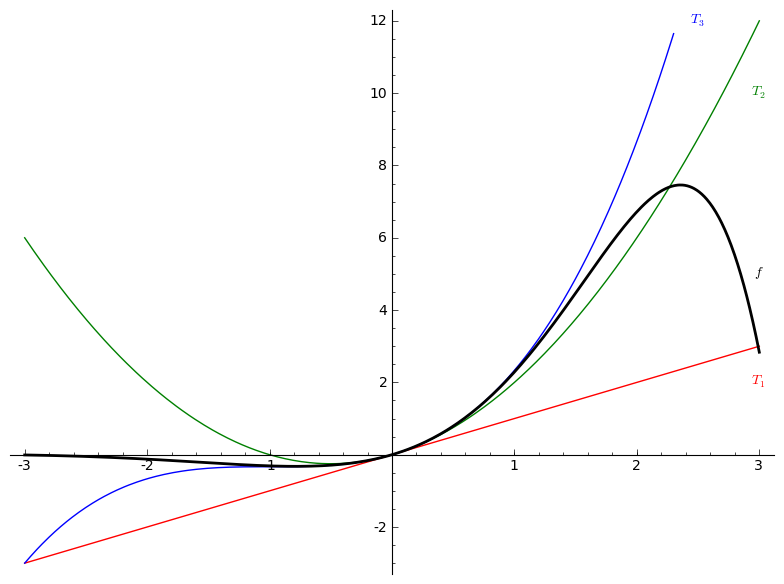
\includegraphics[scale=0.5]{figures/formel-taylor}
\end{center}


\begin{itemize}
  \item Après avoir défini la fonction $f$ par \codeinline{f = sin(x)*exp(x)}, la commande 
  \codeinline{taylor(f,x,0,n)} renvoie le développement limité de
  $f$ en $x=0$ à l'ordre $n$, par exemple ici 
  $f(x) = x + x^2 + \frac13 x^3+ \epsilon(x) x^3$, donc  $T_1(x) = x$,
  $T_2(x)=x+x^2$, $T_3(x) =  x + x^2 + \frac13 x^3$.
  
  \item La commande \codeinline{plot(f,(a,b))} trace le graphe de $f$ sur l'intervalle $[a,b]$.
\end{itemize}


Il est perceptible que :
\begin{itemize}
  \item les polynômes de Taylor sont une bonne approximation de la fonction au voisinage d'un point ;
  \item plus l'ordre du développement limité est élevé, meilleure est l'approximation ;
  \item l'approximation est seulement \emph{locale} : loin du point considéré (ici l'origine),
  les polynômes de Taylor n'approchent plus du tout la fonction.
\end{itemize}

\bigskip

Il est possible de tracer une grande variété de graphiques.
Voici par exemple la courbe de Lissajous d'équation $t \mapsto \big(\cos(3t),\sin(4t)\big)$
et le graphe de la fonction de deux variables définie par 
$f(x,y)= \cos(xy)$.
Les commandes sont :
\begin{itemize}
  \item \codeinline{parametric_plot((cos(3*t),sin(4*t)),(t,0,2*pi))}
  \item \codeinline{plot3d(cos(x*y),(x,-4,4),(y,-4,4))}
\end{itemize}

Attention ! Il faut avoir au préalable défini les variables utilisées : \codeinline{var('t')}
et \codeinline{var('x,y')} (en fait, seule la variable $x$ est définie par défaut dans \Sage).

\begin{center}
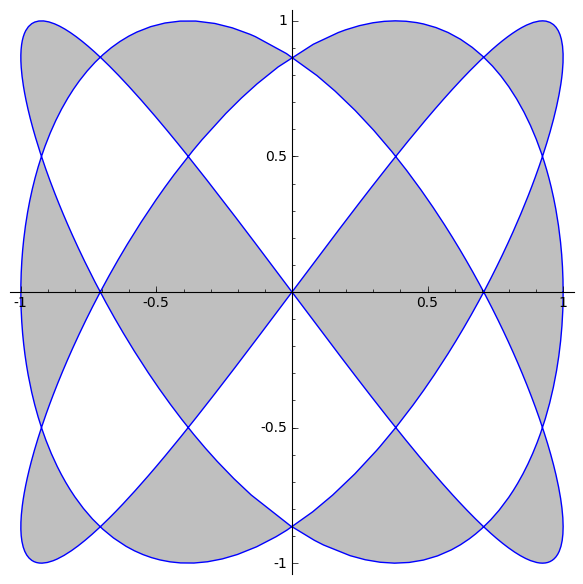
\includegraphics[scale=0.3]{figures/formel-lissajou}
\includegraphics[scale=0.25]{figures/formel-surface}
\end{center}

%--------------------------------------------------------
\subsection{Le calcul formel peut-il tout faire ?}

Le calcul formel ne résout malheureusement pas tous les problèmes 
de mathématique d'un coup de baguette magique !


\begin{tp}
\sauteligne
\begin{enumerate}
  \item Pouvez-vous calculer les solutions réelles de $x^k-x-1=0$ lorsque $k$ est un entier supérieur ou égal à $2$ ?
  \item Est-ce que \Sage\ sait que toutes ces expressions sont nulles ?
  $$2^{10} - 1024 \qquad (x+1)^2-x^2-2x-1 \qquad \sin^2(x)+\cos^2(x) - 1$$
\end{enumerate}  
\end{tp}


\begin{enumerate}
  \item La première limitation est propre aux mathématiques : on ne peut pas trouver 
une écriture explicite des solutions de toutes les équations.
Pour $x^2-x-1=0$, à l'aide de la commande
\codeinline{solve(x^2-x-1==0,x)}, on trouve bien les deux solutions
$\frac{1+\sqrt5}{2}$ et $\frac{1-\sqrt5}{2}$.
Par contre \codeinline{solve(x^5-x-1==0,x)} ne renvoie pas les solutions 
mais l'équation qui définit les solutions (ce qui ne nous avance guère).
Ce n'est pas ici un problème technique de \Sage.
En effet, il n'est mathématiquement pas possible d'exprimer la solution réelle de $x^5-x-1=0$ 
à l'aide de radicaux ($\sqrt{\phantom{0}}, \sqrt{\phantom{0}}, 
\sqrt[3]{\phantom{0}}, \sqrt[4]{\phantom{0}},\ldots$), ceci est seulement possible jusqu'au degré $4$.
Par contre, on obtient une approximation de la solution réelle par la commande 
\codeinline{find_root(x^5-x-1==0,-1,2)} en précisant que l'on 
cherche la solution dans l'intervalle $[-1,2]$.
  
  \item 
  \begin{enumerate}
    \item Sans problème \codeinline{2^10-1024} renvoie $0$.
    \item Il est nécessaire de développer l'expression pour trouver $0$ : \codeinline{expand((x+1)^2-x^2-2*x-1)}.
    \item Il faut explicitement demander de simplifier l'expression trigonométrique :
    d'abord \codeinline{f = sin(x)^2+cos(x)^2 - 1} puis on demande de simplifier \codeinline{f.simplify_trig()}
    pour obtenir $0$.  
  \end{enumerate}
\end{enumerate}

\bigskip

  Il n'est pas du tout évident pour un ordinateur de reconnaître les identités comme $(a+b)^2 = a^2+2ab+b^2$
  ou bien $\cos^2(x)+\sin^2(x)=1$. Souvenez-vous d'ailleurs qu'il faut plusieurs années d'apprentissage 
  pour les assimiler. Lorsqu'il y a plusieurs écritures d'une même expression, 
  il n'est pas non plus évident pour l'ordinateur de savoir quelle forme est la plus adaptée pour l'utilisateur.
  Par exemple, selon le contexte, les trois écritures suivantes sont utiles : $(a-b)^3 = (a-b)(a^2-2ab+b^2)= a^3-3a^2b+3ab^2-b^3$.
  Il faudra donc << guider >> le logiciel de calcul formel avec les fonctions 
  \codeinline{expand}, \codeinline{factor}, \codeinline{simplify}...

\begin{remarque*}
Pour avoir une idée de la difficulté à identifier deux expressions mathématiquement égales, voici 
une représentation de la façon dont sont stockées $(a+b)^2$ et $a^2+2ab+b^2$ dans le logiciel.

\begin{center}
\begin{tikzpicture}

\node (A1) at (0,0) {\texttt{a}};
\node (A2) at (1,0) {\texttt{b}};
\node (B1) at (0.5,1) {\texttt{+}};
\node (B2) at (1.5,1) {\texttt{2}};
\node (C) at (1,2) {\texttt{\^}};

\draw (A1.north) -- (B1.south west);
\draw (A2.north) -- (B1.south east);
\draw (B1.north) -- (C.south west);
\draw (B2.north) -- (C.south east);

\node at (1,-1) {$(a+b)^2$};


\begin{scope}[xshift=5cm]
\node (AA1) at (0,0) {\texttt{a}};
\node (AA2) at (1,0) {\texttt{2}};
\node (AA3) at (2,0) {\texttt{2}};
\node (AA4) at (3,0) {\texttt{a}};
\node (AA5) at (4,0) {\texttt{b}};
\node (AA6) at (5,0) {\texttt{b}};
\node (AA7) at (6,0) {\texttt{2}};
\node (BB1) at (0.5,1) {\texttt{\^}};
\node (BB2) at (3,1) {\texttt{*}};
\node (BB3) at (5.5,1) {\texttt{\^}};
\node (CC) at (3,2) {\texttt{+}};

\draw (AA1.north) -- (BB1.south west);
\draw (AA2.north) -- (BB1.south east);
\draw (AA3.north) -- (BB2.south west);
\draw (AA4.north) -- (BB2.south);
\draw (AA5.north) -- (BB2.south east);
\draw (AA6.north) -- (BB3.south west);
\draw (AA7.north) -- (BB3.south east);

\draw (BB1.north) -- (CC.south west);
\draw (BB2.north) -- (CC.south);
\draw (BB3.north) -- (CC.south east);

\node at (3,-1) {$a^2+2ab+b^2$};
\end{scope}

\end{tikzpicture}
\end{center}
\end{remarque*}
 
  
%--------------------------------------------------------
\subsection{Un peu plus sur \Sage}




Ce cours n'a pas pour but d'être un manuel d'utilisation du logiciel \Sage.
Vous trouverez sur internet des tutoriels pour démarrer et pour un usage avancé : \\
\centerline{\href{http://www.sagemath.org/fr/}{Site officiel de \Sage}}
Il existe aussi un livre gratuit : \\
\centerline{\href{http://sagebook.gforge.inria.fr/}{Calcul mathématique avec \Sage}}

Une façon simple d'obtenir de l'aide pour une commande \Sage\ 
est d'utiliser le point d'interrogation : \codeinline{ln?} (ou bien \codeinline{help(ln)}).
Vous y apprendrez que la fonction \codeinline{ln} est le logarithme naturel.


\bigskip
Il y a deux façons d'utiliser \Sage\ :
\begin{itemize}
  \item \emph{En ligne de commande} : vous obtenez une fenêtre avec l'invite
  \codeinline{sage:} puis vous tapez vos commandes (en n'oubliant pas de faire une copie de
  votre travail dans un fichier texte du type \codeinline{mon_programme.sage}).
  
  \item \emph{Dans votre navigateur} : à partir de l'invite \codeinline{sage:}
  vous tapez \codeinline{notebook()} pour obtenir une interface complète et conviviale.
\end{itemize}

Voici une liste de fonctions usuelles :
\begin{center}
\setlength{\arrayrulewidth}{0.05mm}
%\begin{tabular}{|l|l|l|} \hline
\begin{tabular}[t]{|c|c@{\vrule depth 1.2ex height 3ex width 0mm \ }|} 
\hline
   \codeinline{abs(x)}     &   $|x|$      \\ \hline
   \codeinline{x^n} \  ou \  \codeinline{x**n}     &   $x^n$      \\ \hline
   \codeinline{sqrt(x)}    &  $\sqrt{x}$ \\ \hline   
   \codeinline{exp(x)}     & $\exp x$    \\ \hline   
   \codeinline{ln(x)} \  ou \  \codeinline{log(x)}     & $\ln x$ logarithme népérien \\ \hline
   \codeinline{log(x,10)}  & $\log x$ logarithme décimal \\ \hline
   \codeinline{cos(x), sin(x), tan(x)}  & $\cos x$, $\sin x$, $\tan x$ en radians\\ \hline
   \codeinline{arccos(x), arcsin(x), arctan(x)}  & $\arccos x$, $\arcsin x$, $\arctan x$ en radians \\ \hline      
   \codeinline{floor(x)}  & partie entière $E(x)$ : plus grand entier $n \le x$ (\emph{floor} = plancher) \\ \hline
   \codeinline{ceil(x)}   & plus petit entier $n \ge x$ (\emph{ceil} = plafond) \\ \hline      
\end{tabular} 
\end{center}

Il existe des fonctions spécifiques qui manipulent les entiers, les vecteurs, les matrices, les polynômes, les fonctions mathématiques...
Nous les découvrions au fil des chapitres.

\bigskip

La syntaxe de \Sage\ est celle du langage \Python. 
Il n'est pas nécessaire de connaître ce langage, la syntaxe 
sera introduite au fur et à mesure. Cependant vous pourrez 
étudier avec profit le chapitre <<~\href{http://exo7.emath.fr/cours/livre-algorithmes.pdf}{Algorithmes et mathématiques}~>> du site \href{http://exo7.emath.fr}{Exo7}.

Pour l'instant voici ce que l'on retient de l'exemple donné plus haut :
\insertcode{algos/motiv-calcul-formel-tex2.sage}{motiv-calcul-formel.sage (2)}
\begin{itemize}
  \item Une boucle \codeinline{for n in range(N):} l'indice $n$ parcourt les entiers de $0$ à 
  $N-1$.
  
  \item Le bloc d'instructions suivant \codeinline{print(n, factor(2^(2^n)+1))}
  est donc exécuté successivement pour $n=0$, $n=1$, \ldots $n=N-1$.
  
 \item Les espaces en début de ligne (\emph{l'indentation}) sont essentielles
 car elles délimitent le début et la fin d'un bloc d'instructions.
\end{itemize}

\finchapitre

\end{document}

